\documentclass{beamer}
% Nächstes Auskommentieren um jedes \pause zu 'deaktivieren'!
%\documentclass[handout]{beamer}

\usepackage{talk_BeamerColor}
\usepackage{res/meta/meta}
\usepackage[pantoneblack7,english]{talk_wwustyle_LA}

\usepackage[ngerman]{babel}
\usepackage[utf8]{inputenc}
\usepackage[T1]{fontenc}

% --- Paket um Grafiken im Dokument einbetten zu koennen
\usepackage{graphicx}
\usepackage{caption}
\usepackage{subfigure}
\usepackage{wrapfig}

% --- Pakete fuer mathematischen Textsatz
\usepackage{amsmath}
\usepackage{amssymb}
\usepackage{empheq}
\usepackage{dsfont}		
\usepackage{amstext}
\usepackage{amsfonts}
\usepackage{amsthm}
\usepackage{wasysym}

% --- Paket erweitert deutlich die Verwendung von Farben aus dem Paket 'graphicx'
\usepackage{color}

% --- Paket um Quellcode sauber zu formatieren
\usepackage{listings}

% --- Darstellung von Pseudocode und mehr (algorithmicx packages)
\usepackage{algorithm}
\usepackage{algpseudocode}

%% Physikalisches
\usepackage{nicefrac}
\usepackage{units}
\usepackage{siunitx}
\sisetup{
  inter-unit-product 	=	$\cdot$,
  fraction-function   	= 	\nicefrac,
  load-configurations 	= 	abbreviations,
  per-mode            	= 	fraction,
  separate-uncertainty	=	true,
  output-decimal-marker	=	{.}
  }   
\usepackage{isotope}

%% Aufgabenverwaltung
\usepackage[textwidth=2cm,% Breite der Todo-Eintr�ge
            textsize=footnotesize,% Schriftgr��e der Eintr�ge
            english,% deutsche Beschriftungen
            shadow,% Schlagschatten f�r Boxen (weils so h�bsch ist)
            colorinlistoftodos]{todonotes}% farbige Markierungen f�r unterschiedliche Aufgabentypen
\newcommand{\detail}[1]{\todo[color=Green,inline]{detail: #1}~}% Details k�nnten hinzugef�gt werden
\newcommand{\litcheck}[1]{\todo[color=LightSteelBlue,inline]{refcheck: #1}~}% muss noch einmal �berpr�ft werden
\newcommand{\src}[1][]{\todo[color=Tomato,inline]{reference! #1}~}% Quelle fehlt

% % Zusätzliches:
\usepackage{braket}
\usepackage{epstopdf}
\usepackage{pgfpages}
\usepackage{csquotes}

\newlength{\halftextwidth}
\setlength{\halftextwidth}{\textwidth}
\divide\halftextwidth by 2

% --- Einstellungen

\author{NiMoNa 2016}
\title{Konnektivität im Gehirn}
%\institutelogo{Logo on title frame}
%\institutelogosmall{Logo on other frames}
\subtitle{Lutz Althüser, Tobias Frohoff-Hülsmann, Victor Kärcher,\\ Lukas Splitthoff, Timo Wiedemann}
\date[08.06.2016]{08. Juni, 2016}

% --- Beginn des Dokuments

\begin{document}

\begin{frame}[plain]
	  \maketitle
\end{frame}

\begin{frame}{Überblick}
	  \tableofcontents
\end{frame}

\section{Konnektivität im Gehirn}
\subsection{Einleitung in DCM}
	\begin{frame}{Einleitung in DCM}
		Analyse der effektiven Konnektivität
	\end{frame}
	
\subsection{Modell}
	\subsubsection{Bilineraes Modell}
	\begin{frame}{Bilineares Modell}
		neuronales Modell der Verbindungen bestimmter Hirnregionen
		Gehirn als nicht-lineares, deterministisches, dynamisches System 
		\begin{figure}[H]
			\begin{center} \label{fig: bilinearesModell}
				\includegraphics[scale=0.4]{bilinearesModell.eps}
				\caption{Bilineares Modell der Netzwerkgröße 3}
			\end{center}
		\end{figure}		
			
		\textbf{Annahme:}
		\begin{itemize}
			\item direkter Einfluss: Eingangssignal $ u_1 $ $ \rightarrow $ Veränderung von Zustandsvariablen (z.B. neuronaler Aktivität)
			\item indirekter Einfluss: Eingangssignal $ u_2 $ $ \rightarrow $ Veränderung der eff. Konnektivität
		\end{itemize}
			
	\end{frame}
	\subsubsection{Hemodynamisches Modell}
	\begin{frame}{Hemodynamische Modell}
		\[\dot{z}=(A+\sum_{j}u_jB^j)z+Cu\]
		  \[
		 A=\left(\begin{array}{ccc} 
		  a_{11} &  a_{12} & a_{13} \\a_{21} &  a_{22} & a_{23} \\a_{31} &  a_{32} & a_{33}
		  \end{array}\right) 
		  \]
		  \[
		  B=\left(\begin{array}{ccc} 
		  b_{11} &  b_{12} & b_{13} \\b_{21} &  b_{22} & b_{23} \\b_{31} &  b_{32} & b_{33}
		  \end{array}\right) 
		  \]
		  \[
		  C=\left(\begin{array}{cc} 
		  c_{11} &  c_{12} \\c_{21} &  c_{22} \\c_{31} &  c_{32} 
		  \end{array}\right) 
		  \]
	\end{frame}

\section{Numerische Algorithmen}
\subsection{Euler-Verfahren}
	\begin{frame}{Euler-Verfahren}
		explizites Verfahren
	\end{frame}
	
\subsection{Runge-Kutta-Verfahren (4. Ordnung)}
	\begin{frame}{Runge-Kutta-Verfahren (4. Ordnung)}
		Analyse der effektiven Konnektivität
	\end{frame}

\section{DCM-Experimente}
\subsection{linear}
	\begin{frame}{Numerisches Experiment - linear}
		Analyse der effektiven Konnektivität
	\end{frame}
\subsection{bilinear}
	\begin{frame}{Numerisches Experiment - bilinear}
		Analyse der effektiven Konnektivität
	\end{frame}
\subsection{hemodynamisch}
	\begin{frame}{Numerisches Experiment - hemodynamisch}
		Analyse der effektiven Konnektivität
	\end{frame}

\section{Literatur}
	\begin{frame}{Literatur}
		\begin{itemize}
			\item 1
		\end{itemize}
	\end{frame}



\begin{frame}
	\frametitle{Designfeatures}
	\begin{block}{Hervorhebungen}
	 \textbf{Wenn man Dinge hervorheben möchte nutzt man entweder Fettdruck,} \textit{ kursive Schrift} \alert{ oder das Schlüsselwort "alert"}. Auch "itemize"-Umgebungen werden von der Stilvorlage überschrieben:
	\end{block}
	\pause
	\begin{itemize}
	 \item So wird sichergestellt,
	 \item dass alle Elemente der Präsentation 
	 \item dieselbe Farbe nutzen.
	\end{itemize}
	\begin{alertblock}{Achtung!}
	 Hier kommt Rot ins Spiel!	
	\end{alertblock}
	\begin{exampleblock}{Beispiel}
	 Hier kommt Grün ins Spiel!
	\end{exampleblock}
\end{frame}

\end{document}
